

\section{Definition of simulation scenarios}

In this section the simulation scenarios and settings are described to get a complete picture of the simulated cloud environment. 

The simulation scenarios can be divided into two parts which are day ahead and real time simulations based on day ahead and real time energy prices, respectively. For each type of simulation different locations and energy markets have been chosen. The basic scenario types are oulined below. 


\subsection{Day ahead simulation scenario}

The simulation scenario for day ahead energy prices is comprised of data centers located in Europe and the USA. A map showing five data centers as a basis for day ahead simulations is outlined in Figure \ref{fig:usa_europe_map}. 

\begin{figure}[htbp]
	\centering
		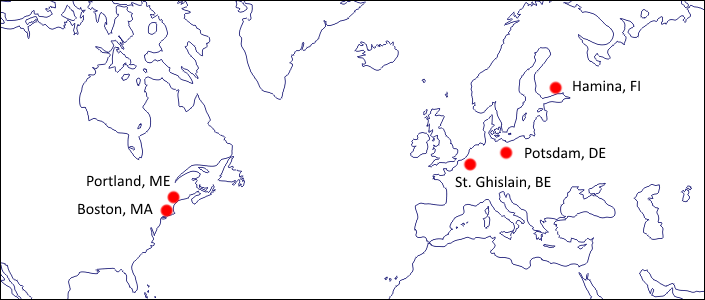
\includegraphics[width=0.7\textwidth]{figures/evaluation_and_results/usa_europe_map.png}
	\caption{Map of data center locations for day ahead price simulations}
	\label{fig:usa_europe_map}
\end{figure}

The locations have been chosen such that a diverse set of data from different energy markets is available. In addition time zone effects should be modeled by placing data centers sufficiently far from each other such that daily variation of energy prices in different time zones can be utilized. 

A list of day ahead energy markets and corresponding locations is shown in Table \ref{tab:list_of_day_ahead_markets}. 


\begin{table}[htbp]
\centering
\begin{tabular}{ll}
\toprule
 Energy market & Location \\
\midrule
	Nord Pool Spot &  Hamina, Finland \\
	Belpex &  St. Ghislain, Belgium \\
	EPEXSpot &  Potsdam, Germany \\
	ISO New England &  Portland, Maine \\
	ISO New England &  Boston, Massachussetts \\
\bottomrule
\end{tabular}
\caption{List of day ahead energy markets and locations}
\label{tab:list_of_day_ahead_markets}
\end{table}




\subsection{Real time simulation scenario}

For the real time simulation scenario data centers have been chosen exclusively from location within the US. Thus energy prices are more localized and performance of simulations should be evaluated for datasets with similar characteristics in contrast to day ahead simulations. 

A map showing data centers for all real time markets and locations is depicted in Figure \ref{fig:usa_map}. 

\begin{figure}[htbp]
	\centering
		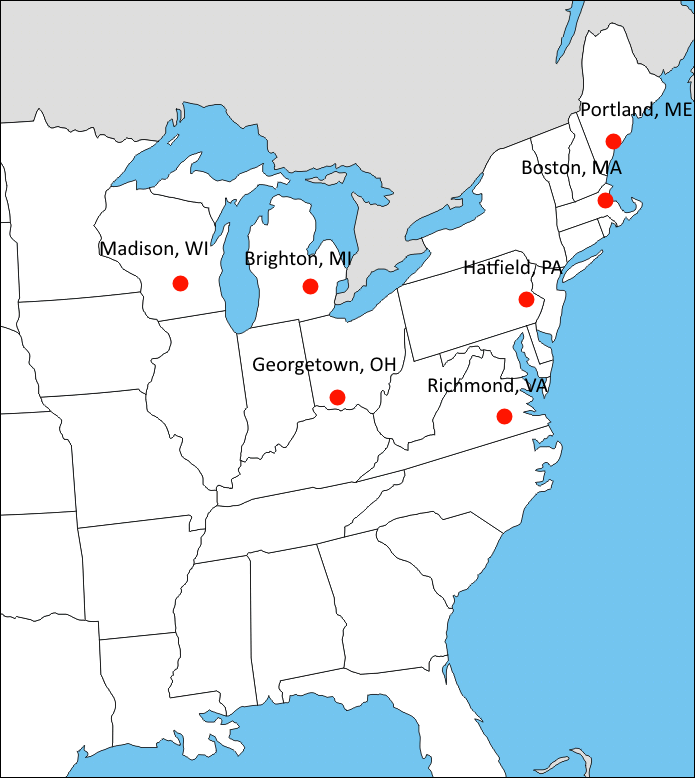
\includegraphics[width=0.50\textwidth]{figures/evaluation_and_results/usa_map.png}
	\caption{Map of data center locations for real time price simulations}
	\label{fig:usa_map}
\end{figure}

A list of real time energy markets and locations is outlined in Table \ref{tab:list_of_real_time_markets}. 

\begin{table}[htbp]
\centering
\begin{tabular}{ll}
\toprule
 Energy market & Location \\
\midrule
	ISO New England &  Portland, Maine \\
	ISO New England &  Boston, Massachussetts \\
	PJM & Richmond, Virginia  \\
	PJM & Brighton, Michigan  \\
	PJM & Hatfield, Pennsylvania  \\
	PJM & Madison, Wisconsin  \\
	PJM & Georgetown, Ohio  \\
\bottomrule
\end{tabular}
\caption{List of real time energy markets and locations}
\label{tab:list_of_real_time_markets}
\end{table}





\subsection{Simulation Configuration Parameters}

\subsubsection{Cloud settings}

As the simulator has been built to be highly configurable \cite{lucanin2015philharmonic} different cloud parameters can be adjusted to run simulations with different settings. In Table \ref{tab:list_of_cloud_metrics} the most relevant simulation parameters are listed. 

\begin{table}[htbp]
\centering
\begin{tabularx}{\textwidth}{l|l|X}
	Metric & Values & Description \\
\hline
	number of servers & 500 & The total number of servers across all locations \\
	number of virtual machines & 5000 & The total number of virtual machines over the whole simulation time period \\
	server cpus & $[4,8]$ & The number of CPUs per server uniformly distributed over the given interval \\
	server memory & $[8,16]$ & The amount of memory per server uniformly distributed over the given interval \\
	virtual machine cpus & $[1,4]$ & The number of CPUs per VM uniformly distributed over the given interval \\
	virtual machine memory & $[1,4]$ & The amount of memory per VM uniformly distributed over the given interval \\
	dirty page rate & $\{20,40,70,90\}$ & One of four dirty page rates in MB/s assigned to each VM \\
	SLA level & 99.95\% & A fixed SLA availability level applied to each VM \\
	VM duration & $\{1,2,5,8,12,24,48\}$ & A fixed set of duration values in hours applied uniformly to the set of VMs \\
	VM price & 4 \cent \ / h & The price of a VM in cent per hour \\
	bandwidth & $\{400,800,1000\}$ & One of 3 amounts of bandwidths in MBit/s set between each two locations \\
	bandwidth cost & 0.1 \cent \ / GB & Bandwidth costs in cent per GB \\
	server peak power & 200 W & The power a server draws when its resources are fully utilized \\
	server idle power & 100 W & The power a server draws when idle \\
	cpu resource weight & 0.7 & The weight associated with cpu power when calculating server utilization \\
	memory resource weight & 0.3 & The weight associated with memory when calculating server utilization \\
\end{tabularx}
\caption{List of cloud metrics in the simulation}
\label{tab:list_of_cloud_metrics}
\end{table}

The number of servers and VMs per simulation has been adjusted such that the resulting utilization is reasonable, e.g.~with 1000 servers and 2000 VMs in total an average utilization of only about 1 \% has been achieved over a simulation period of 5 weeks. Thus raising the number of VMs and in turn reducing number of servers led to a more realistic utilization of 30\% to 40\%. 

The relation of number of resources per server to the amount of VM resources (i.e.~number of cpus, memory) has been defined such that capacity constraints will not be an issue in simulations. The same method has been applied to the relation of total number of servers to number of VMs. 

The dirty page rate has a direct impact on VM migration performance (see Section \ref{sec:modeling_migration_energy}) and therefore different values have been assigned to VMs to simulate different application behavior. In combination with bandwidth this may lead to a high variation in migration downtimes. 

The SLA level has been set to the most common value for internet cloud services \cite{google2015compute,amazon2013sla}. With different penalty levels greater downtimes directly impact resulting costs for cloud providers. 

A different set of duration values has been assigned to VMs in order to simulate different kinds of workloads. This includes VM durations of 1 to 48 hours for scientific or HPC applications. Long running VMs have been omitted to focus on short term applications. 

The VM price most resembles the price for a ``n1-standard-1'' VM on Google Compute Cloud\footnote{\url{https://cloud.google.com/compute/pricing}}. As this is one of the smallest VMs available in the Google Cloud this price is still comparably cheap. 

Bandwidth is divided into low, medium and high values to simulate real world scenarios where high bandwidth may not always be available. As bandwidth has a direct impact on migration downtime this allows to evaluate the total resulting downtime and costs in different scenarios. 

Bandwidth costs have been set to a fixed price per amount of traffic while it is usually paid by fixed price contracts with 95/5 bandwidth constraints \cite{qureshi2009cutting}. These contracts measure traffic in fixed time intervals and the 95-th percentile of total usage is charged. To simplify the model in this work it has been set to a fixed price per volume. 

Server peak and idle power have been set where a server at peak load consumes double the amount of power than when idle. This may be too optimistic as it is stated that servers consume about 60\% of power when idle \cite{meisner2009powernap}. However studies show that new server technology is able to achieve power reductions up to 75\% from peak to idle mode \cite{prime2011energy}. 
A greater ratio of peak to idle power results in greater possibility for energy savings. Therefore the idle-to-peak ratio is critical for any scheduling algorithms aiming to reduce costs based on energy. 

CPU and memory resource weights have been defined to calculate resulting power consumption from server utilization of each resource. From investigations in \cite{meisner2009powernap,kansal2010virtual} it can be deduced that CPU is the most power consuming component where memory power consumption amounts to about one third up to equal amounts of CPU power. Therefore CPU and memory weights have been set to accommodate those findings. 



\subsubsection{Cost models}

Cost models and related metrics are an important base for transforming aggregated power values to actual costs. Therefore a number of formulas have been defined to accurately model the resulting power consumption and energy costs. 
%These formulas are outlined below. 

\paragraph{Utilization of servers}
The basis for modeling power consumption is to define resource utilization of servers since server utilization relates directly to resulting power consumption \cite{meisner2009powernap}. 
Server utilization based on a set of resources $R$ is defined in Equation \ref{eq:server_utilization}. 

\begin{equation}
	s_{util}(t) = \sum_{r \in R} w_r \frac{s_{used}(r,t)}{s_{cap}(r)}
	\label{eq:server_utilization}
\end{equation}

with $w_r$ denoting the weight of resource $r$, $s_{used}$ is the currently used capacity of server $s$ regarding resource $r$ at time $t$, $s_{cap}$ denotes the total capacity of server $s$ of resource $r$ and $s_{util}$ being the resulting utilization of the server. 


\paragraph{Utilization per location}
In order to calculate data center load for each location a method of computing the average utilization per location is needed. 
It is defined as the average utilization of all servers in a given location (Equation \ref{eq:utilization_per_location}): 

\begin{equation}
	util_{loc}(t) = \frac{1}{|loc_{s}|} \sum_{s \in loc_{s}} s_{util}(t)
\label{eq:utilization_per_location}
\end{equation}

where $loc_{s}$ being the set of servers at location $loc$ and $util_{loc}$ denotes the current utilization at location $loc$. 


\paragraph{Power per location}

From the previous metric \textit{utilization per location} the resulting cloud power per location can be derived (Equation \ref{eq:power_loc}). 

\begin{equation}
	power_{loc}(t) = util_{loc}(t) \cdot |loc_{active_s}(t)| \cdot (P_{peak} - P_{idle}) + |loc_{active_s}(t)| \cdot P_{idle}
\label{eq:power_loc}
\end{equation}

where $|loc_{active_s}(t)|$ is the number of active servers at location $loc$ at time $t$, $P_{peak}$ is the peak power of the server and $P_{idle}$ describes the idle power of the server. 

\paragraph{Total cloud power}

The total cloud power is the sum of power consumption over all locations $L$ and time periods $T$ (Equation \ref{eq:m_tcp}). 

\begin{equation}
	m_{TCP} = \sum_{t \in T} \sum_{loc \in L} power_{loc}(t)
\label{eq:m_tcp}
\end{equation}


\paragraph{Migration load}
This metric serves as the basis for calculating migration energy as it directly depends on migration load. In addition it is used for further metrics such as migration costs. The formula for aggregated migration load per time $t$ is outlined in Equation \ref{eq:migration_load}.

\begin{equation}
	mig_l(t) = \sum_{v \in VM} V_{mig}(v,t)
\label{eq:migration_load}
\end{equation}

where $VM$ denotes the set of all active VMs at time $t$ and $V_{mig}(v,t)$ is the total migration load for vm $v$ for a migration starting at time $t$. The latter expression is taken from the definition of migration energy in Section \ref{sec:modeling_migration_energy}. 

\paragraph{Migration energy}
Modeling migration energy is needed for calculating the migration costs and it may also give a hint for resulting downtime and possible penalty costs due to the amount of migration energy consumed. 
The formulas for summed migration energy over the set of all VMs $VM$ and total migration energy over a simulation time period are denoted in Equations \ref{eq:migration_energy_by_time} and \ref{eq:migration_energy_total}. 

\begin{align}
	mig_e(t) = \sum_{v \in VM} E_{mig}(v,t) \label{eq:migration_energy_by_time}\\
	m_{ME} = \sum_{t \in T} mig_e(t) \label{eq:migration_energy_total}
\end{align}

\paragraph{Migration cost}
The migration costs are defined on the one side by combining resulting migration energy with current energy prices and on the other side by combining migration load and bandwidth costs. 

\begin{align}
	p_{mean}(t) &= \frac{p_{l1}(t) + p_{l2}(t)}{2} \label{eq:p_mean} \\
	mig_c(t) &= mig_e(t) \cdot p_{mean}(t) \label{eq:mig_c} \\
	mig_{c_{bw}}(t) &= mig_l(t) \cdot c_{bw} \label{eq:mig_c_bw} \\
	m_{MC} &= \sum_{t \in T} \left( mig_c(t) + mig_{c_{bw}}(t) \right) \label{eq:m_mc} 
\end{align}

Equation \ref{eq:p_mean} shows the mean price calculated from prices $p_{l1}$ and $p_{l2}$ in locations $l1$ and $l2$ at time $t$. 
Equation \ref{eq:mig_c} describes the migration costs depending on the migration energy and mean energy price $p_{mean}$ at time $t$. 
The bandwidth related costs for migration are outlined in Equation \ref{eq:mig_c_bw} with migration load and bandwidth costs combined (i.e.~amount of GB multiplied by \cent \ / GB). The migration cost metric $m_{MC}$ in Equation \ref{eq:m_mc} is then the sum of both energy and bandwidth costs. 

\paragraph{Cost of VM}
The resulting costs $v_c$ for a user of a VM is defined as the price $v_p$ set for the VM multiplied by its duration up to time $t$ (Equation \ref{eq:cost_of_vm}). 

\begin{equation}
	v_c(t) = v_p \cdot v_{dur}(t)
\label{eq:cost_of_vm}
\end{equation}

\paragraph{Penalty cost}

The total penalty costs are the aggregated costs for all penalties and VMs occurred during a simulation. Penalty costs occur when the maximum allowed downtime for a VM regarding an SLA threshold is exceeded. Depending on the threshold that has been surpassed different penalty costs have to be paid. 
As described in Section \ref{sec:sla_managemenet} three different penalty thresholds are defined which result in different penalty costs. 

\begin{align}
	SLA_{TH_i}(v,t) &= v_{dur}(t) \left( 1 - \frac{v_{SLA_i}}{100} \right), i \in \{1,2,3\} \label{eq:sla_th_i} \\
	v_{SLA_1} &= 99.95, v_{SLA_2} = 99, v_{SLA_3} = 95 \label{eq:sla_levels} \\
	v_{pen}(t) &= \left\{
								\begin{array}{@{}ll@{}}
									0.5, & \text{if } down_{acc}(v,t) > SLA_{TH_3}(v,t) \\
									0.25, & \text{if } down_{acc}(v,t) > SLA_{TH_2}(v,t) \\
									0.1, & \text{if } down_{acc}(v,t) > SLA_{TH_1}(v,t) \\
									0, & \text{otherwise}
								\end{array}\right. \label{eq:v_pen}  \\
	v_{c_{pen}}(t) &= v_c(t) \cdot v_{pen}(t) \label{eq:v_c_pen} \\
	m_{TPC} &= \sum_{v \in VM} v_{c_{pen}}(t_{last}) \label{eq:m_pc} 
\end{align}

Equation \ref{eq:sla_th_i} defines an SLA threshold for either of the defined SLA levels in Equation \ref{eq:sla_levels}. In Equation \ref{eq:v_pen} penalty values in the interval [0,1] are assigned based on the SLA threshold reached. This penalty value is then applied to the costs of the VM in Equation \ref{eq:v_c_pen} resulting in penalty costs for VM $v$. Equation \ref{eq:m_pc} calculates the total penalty costs across all VMs at the last simulation time stamp $t_{last}$. 


\paragraph{Total downtime}

The total downtime is calculated from the sum of downtimes of all VMs over the whole simulation time period (up to $t_{last}$, Equation \ref{eq:m_tdt}). 

\begin{equation}
	m_{TDT} = \sum_{v \in VM} down_{acc}(v,t_{last})
\label{eq:m_tdt}
\end{equation}

\paragraph{Number of migrations}

The total number of migrations is defined as the sum of migrations at each time stamp $t$ (Equation \ref{eq:num_migrations}). 

\begin{equation}
	m_{NM} = \sum_{t \in T} mig_{num} (t) 
\label{eq:num_migrations}
\end{equation}

where $mig_{num}(t)$ denotes the number of migrations at time $t$. 


\paragraph{Total cloud costs}

The total cloud costs are calculated as the sum of cloud power values multiplied by the price at the respective location and time (Equation \ref{eq:m_tcc}). 

\begin{equation}
	m_{TCC} = \sum_{t \in T} \sum_{loc \in L } power_{loc}(t) \cdot p_{loc}(t)
\label{eq:m_tcc}
\end{equation}

\paragraph{Total cloud power with migrations}

Calculating the total cloud power including migrations is a simple addition of the total cloud power and migration energy (Equation \ref{eq:m_tcpwm}). 

\begin{equation}
	m_{TCPWM} = m_{TCP} + m_{ME}
\label{eq:m_tcpwm}
\end{equation}

\paragraph{Total cloud cost with migrations}

Analogously to \textit{Total power with migrations} this metric is defined as the sum of total cloud cost and migration cost (Equation \ref{eq:m_tccwm}). 

\begin{equation}
	m_{TCCWM} = m_{TCC} + m_{MC}
\label{eq:m_tccwm}
\end{equation}

\paragraph{Total power}

The total power metric encompasses the metric \textit{Total cloud power with migrations} to describe the total power consumption in the simulation (Equation \ref{eq:m_tp}). 

\begin{equation}
	m_{TP} = m_{TCPWM}
\label{eq:m_tp}
\end{equation}

\paragraph{Total cost}

Total cost denote the sum of all cost occurred during simulation which includes the total cloud cost with migrations plus total penalty costs (Equation \ref{eq:m_tc}). 

\begin{equation}
	m_{TCCWM} = m_{TCCWM} + m_{TPC}
\label{eq:m_tc}
\end{equation}


\section{Utility function optimization}


\section{Simulation Results}

A detailed presentation of the simulator and scheduler that actually run through the simulation scenarios is given in this section. Then the results from the simulation runs based on different settings and data is presented and scenarios are compared to evaluate the most promising approach in the defined setting. Finally the results are discussed and evaluated to draw conclusions about the possible performance gains when running these scenarios, and how much they differ from the optimal solution. 

%%% final , summarized %%%




\subsection{Total costs}


\begin{table}[ht]
\centering

\begin{tabular}{lrrrrrrr}
\toprule
{} &     BFD &     BCU &   BCU\_F &  BCU\_IF &   BCU\_M &  BCU\_MF &  BCU\_MIF \\
\midrule
DA Summer &  208.36 &  181.72 &  171.85 &  174.53 &  186.19 &  \textbf{169.86} &   173.29 \\
RT Summer &  315.96 &  263.32 &  265.21 &  256.08 &  273.87 &  259.98 &   \textbf{252.09} \\
DA Spring &  930.41 &  630.13 &  592.83 &  600.42 &  625.62 &  \textbf{585.97} &   595.81 \\
RT Spring &  966.04 &  710.59 &  659.92 &  699.13 &  747.06 &  \textbf{647.57} &   668.35 \\
\bottomrule
\end{tabular}
\caption{Total costs for different scenarios (in \$)}
\end{table}

\begin{table}[ht]
\centering
\begin{tabular}{lrrrrrrr}
\toprule
{} &  BFD &    BCU &  BCU\_F &  BCU\_IF &  BCU\_M &  BCU\_MF &  BCU\_MIF \\
\midrule
DA Summer &    0 &  12.79 &  17.52 &   16.24 &  10.64 &   \textbf{18.48} &    16.83 \\
RT Summer &    0 &  16.66 &  16.06 &   18.95 &  13.32 &   17.72 &    \textbf{20.21} \\
DA Spring &    0 &  32.27 &  36.28 &   35.47 &  32.76 &   \textbf{37.02} &    35.96 \\
RT Spring &    0 &  26.44 &  31.69 &   27.63 &  22.67 &   \textbf{32.97} &    30.82 \\
\bottomrule
\end{tabular}
\caption{Normalized total cost reductions for different scenarios (in \%)}
\end{table}





